%\documentclass{article}
%\usepackage{graphicx,subfigure}
%\usepackage{caption,rotating}
%\begin{document}

\begin{figure}[p]
\centering
 \subfigure[Subfigure (i) Flock No 1 of Trial 2]{
%   \label{fig:redpixt2(i)}
    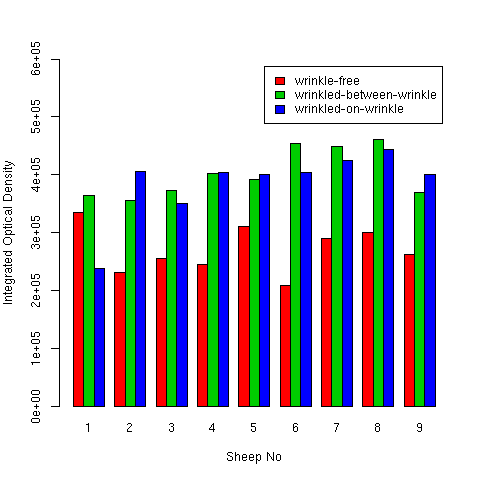
\includegraphics[scale=0.50]{t2f1odmeans.png}
% 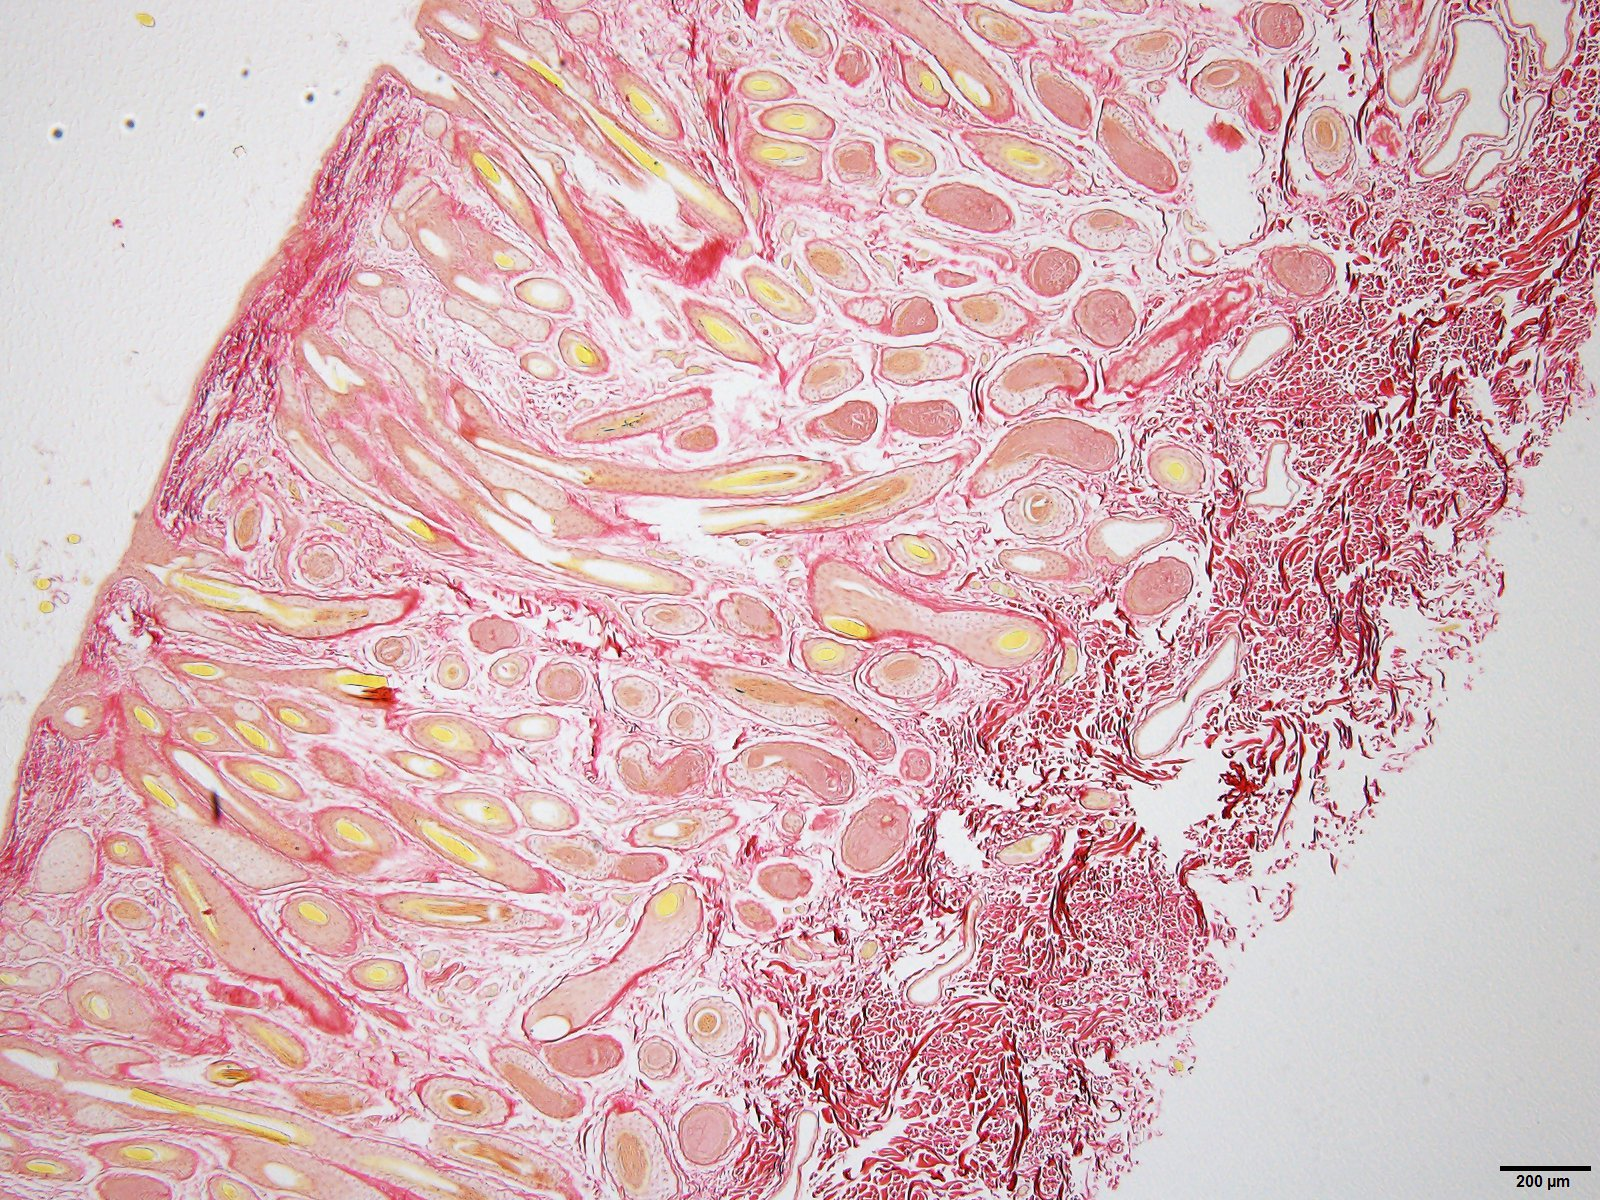
\includegraphics[width=1.0\textwidth]{w479-2-rigid.jpg}
  }
 \subfigure[Subfigure (ii) Flock No 2  of Trial 2]{
%   \label{fig:redpixt2(ii)}
    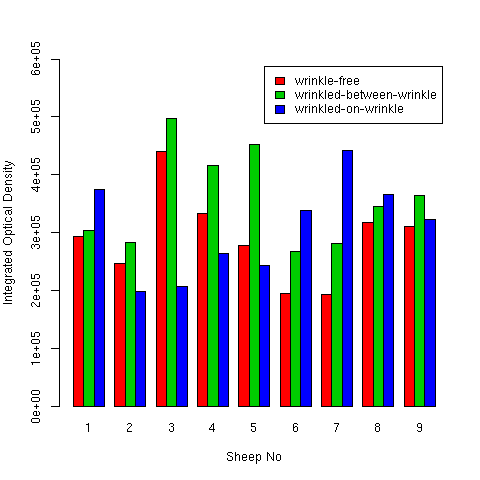
\includegraphics[scale=0.50]{t2f2odmeans.png}
  }
  \caption{Integrated optical density of the red images of sections stained with PSR for each of the nine sheep in each Flock of Trial 2, averaged over five microscope fields}
\vfill
  \label{fig:redpixt2}
\end{figure}

%\end{document}

